\documentclass[a4paper, 12pt]{article}
\usepackage[utf8]{inputenc}
\usepackage[T1]{fontenc}
\usepackage[magyar]{babel}
\usepackage{graphicx}
\usepackage[margin=65 pt]{geometry}
\usepackage{amsmath}
\usepackage{wrapfig}


\begin{document}

\begin{titlepage}\centering
\vspace*{250 pt}
\Huge \textbf{Folytonos közegek mechanikája}

\LARGE \textbf{1. tétel}

\LARGE Egyszerű deformációk, nyújtás, haránt összehúzódás, nyírás


~

\LARGE Kidolgozta: Pollák Edina

\vspace*{\fill}
\end{titlepage}

\newpage
\part*{\Large{}}

\vspace{30 pt}

Az első félévben merev testekkel dolgoztunk, ezek pontjainak távolsága nem változhat meg. Ebben a félévben viszont olyan testekkel fogunk foglalkozni amikre ez nem igaz, tehát nem lehet majd leírni a testek mozgását a megszokott 6 egyenlettel. Ahogy mechanika előadásokon már megfigyelhettük, itt is kísérleti tapasztalat alapján írjuk majd le a testek viselkedését.

~

\subsection*{Első kísérlet: Rézdrót nyújtása}

~

\begin{figure}[h]
\centering
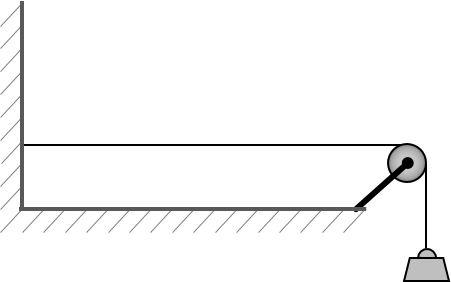
\includegraphics[scale=0.5]{tetel1_1.png}
\caption{}
\end{figure}

        Egy rézdrótot egyik végénél rögzítünk, a másik végén pedig elkezdjük terhelni (1 ábra). A dróton         elhelyezünk egy markert, és megfigyeljük, ahogy elmozdul a terhelés változtatásával, ez a drót megnyúlását hivatott reprezentálni. Azt figyelhetjük meg, hogy egy bizonyos terhelésig a nyújtás reverzibilis, tehát megszűnésére a drót visszanyeri eredeti alakját. Eddig a bizonyos határig azt figyelhetjük meg, hogy a nyúlás és a terhelő erő között lineáris összefüggés van (kristályos anyagoknál). 
        
        Ezt a határt (folyáshatárt) átlépve, a megnyúlás már nem visszafordítható, ha megszüntetjük a terhelést, csökken a hossz egy lineáris görbe mentén, ami az előzővel párhuzamos, de van maradandó deformáció (2. ábra). A gumi nyújtásánál a görbe nem lineáris, viszont az alakváltozás reverzibilis.
        
\begin{figure}[h]
\centering
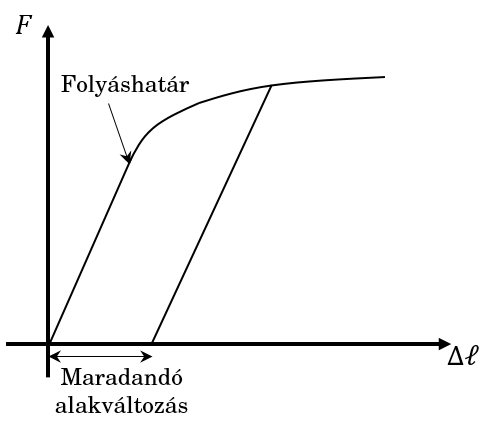
\includegraphics[scale=0.5]{tetel1_2.png}
\caption{}
\end{figure}

A megnyúlás arányos a kezdeti hosszal, ezért érdemes a relatív megnyúlás, deformáció, fogalmát bevezetni. $\varepsilon=\frac{\Delta\ell}{\ell}$, mely egy mértékegység nélküli érték. 

Az erő pedig a keresztmetszettel arányos, ezért bevezetjük a rugalmas feszültséget $\sigma=\frac{F}{A}$, melynek mértékegysége $\mathrm{Pa}$. 

\begin{figure}[h]
\centering
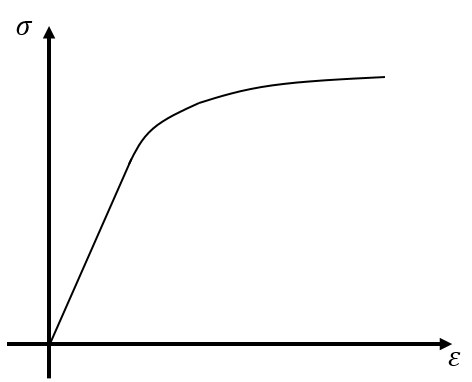
\includegraphics[scale=0.5]{tetel1_3.png}
\caption{}
\end{figure}

A két újonnan bevezetett változó alkalmasabb számolásokra, hiszen nem függenek a test geometriájától, az anyagok minőségét jellemzik. Rugalmas esetben arányosak:

$$\sigma=E\varepsilon$$ 
 
Ez a Hooke-törvény, az arányossági tényező ($E$) a Young-modulus. 

~

A Young-modulus anyagra jellemző állandó, nagyságrendileg $100~ \mathrm{GPa}$ minden anyagra. Kísérleti tapasztalat alapján, a test $100~\mathrm{MPa}$ feszültség esetén maradandó alakváltozást szenved, a deformáció $10^-3$ nagyságrendű ($\varepsilon$ kicsi).

~

~




\subsection*{Második kísérlet: Gumi nyújtása(haránt összehúzódás)}

~

Gumiszál megnyújtása esetén a keresztmetszete csökken, és a kísérleti tapasztalat alapján a relatív átmérőváltozás arányos a deformációval
            
$$\frac{\Delta d}{d}=-\nu\frac{\Delta\ell}{\ell}$$

ahol a $\nu$ a Poisson-szám.

~

Felvehet negatív értéket, de nem lehet akármekkora, többnyire $0,3\pm 0,1$ intervallumon belül található.

~

~

\subsection*{Relatív térfogatváltozás}


Összenyomás során a hossz és a keresztmetszet változik, így a test térfogata is. Közelítsük az alakváltozást szenvedő testet egy $d$ alapélű és $\ell$ magasságú négyzetes hasábbal. Habár megjegyzendő, hogy az alábbiakban levezetett azonosságok más alakú testek esetén érvényesek. Ekkor a relatív térfogatváltozás:

$$\frac{\Delta V}{V}=\frac{(d+\Delta d)^2(\ell+\Delta\ell)-\ell d^2}{\ell d^2}=\frac{(d^2+2d\Delta d+\Delta d^2)(\ell+\Delta\ell)-\ell d^2}{\ell d^2}$$

$$\frac{\Delta V}{V}=\frac{2d\Delta d\ell+\Delta d^2\ell+2d\Delta d\Delta\ell+\Delta d^2\Delta\ell+d^2\Delta\ell}{\ell d^2}$$

Mivel $\Delta d^2$ és $\Delta d\Delta\ell$ a kísérleti tapasztalat alapján kicsik, az olyan tagok, amikben előfordulnak, elhanyagolhatóak:

$$\frac{\Delta V}{V}\approx \frac{2\ell d\Delta d+d^2\Delta\ell}{\ell d^2}=2\frac{\Delta d}{d}+\frac{\Delta\ell}{\ell}$$

A Hooke-törvényt, és a haránt megnyúlás azonosságát felhasználva:

$$\frac{\Delta V}{V}=(1-2\nu)\frac{\Delta\ell}{\ell}=(1-2\nu)\frac{\sigma}{E}$$

Folyadékokban és gázokban, ahol a rugalmas feszültséget a nyomás helyettesíti, ez a következőképp írható:

$$\frac{\Delta V}{V}=-3\frac{1-2\nu}{E}p$$

A háromszoros szorzó a három irány miatt jelenik meg, ahonnan a nyomás hat, a negatív előjel pedig a nyomás definíciója miatt (pozitív nyomás esetén általában térfogatcsökkenés lép fel). A kapott egyenletből az arányossági tényezőre bevezetjük a kompresszibilitást:

$$\kappa=\frac{3(1-2\nu)}{E}$$

majd a kompresszió modulust: 

$$K=\frac{1}{\kappa}=\frac{E}{3(1-2\nu)}$$

Fontos következmény, hogy ha $\nu>0,5$, akkor $\kappa<0$, az anyag összenyomás hatására kitágul, felrobban. Emiatt stabil rendszerekre $\nu<0,5$.



\end{document}